\documentclass{beamer}
\usepackage{media9}
%\usepackage{movie15}


%\usepackage{graphicx}
\usepackage{verbatim}

\useoutertheme{shadow}
%\usecolortheme{orchid}
\usecolortheme{seahorse}

\renewcommand{\a}{\alpha}
\renewcommand{\b}{\beta}
\renewcommand{\d}{\delta}
\newcommand{\g}{\gamma}
\newcommand{\s}{\sigma}
\newcommand{\w}{\omega}
\renewcommand{\k}{\vec{k}}
\newcommand{\td}[1]{\tilde{#1}}
\newcommand{\x}{\vec{x}}
\newcommand{\p}{\phantom{\alpha}}

\def\toonscale{0.45}
\def\mboxy#1{\mbox{\small #1}}


\begin{comment}
\AtBeginSection[]{
  \frame{
    \frametitle{Outline}
    \tableofcontents[currentsection]
  }
}
\end{comment}

\title{Galaxy Angular Momentum}
\subtitle{History, Framework}
\author[Boyle and Pen]{Ue-Li Pen \\[8mm] 
}
\date{SJTU, October 21, 2019}


\begin{document}

\frame{\titlepage}

%\section*{Introduction}
\section{Introduction}

\begin{comment}
  \subsection{Outline}

  \frame{
    \frametitle{Outline}
    \tableofcontents
  }
\end{comment}

\subsection{History}
  \frame{
    \frametitle{Centuries}
    \begin{itemize}
      \item GAMA pioneers:
      \item G\"odel 1949, Peebles 1969, 1971, SDM White 1984
    \end{itemize}
     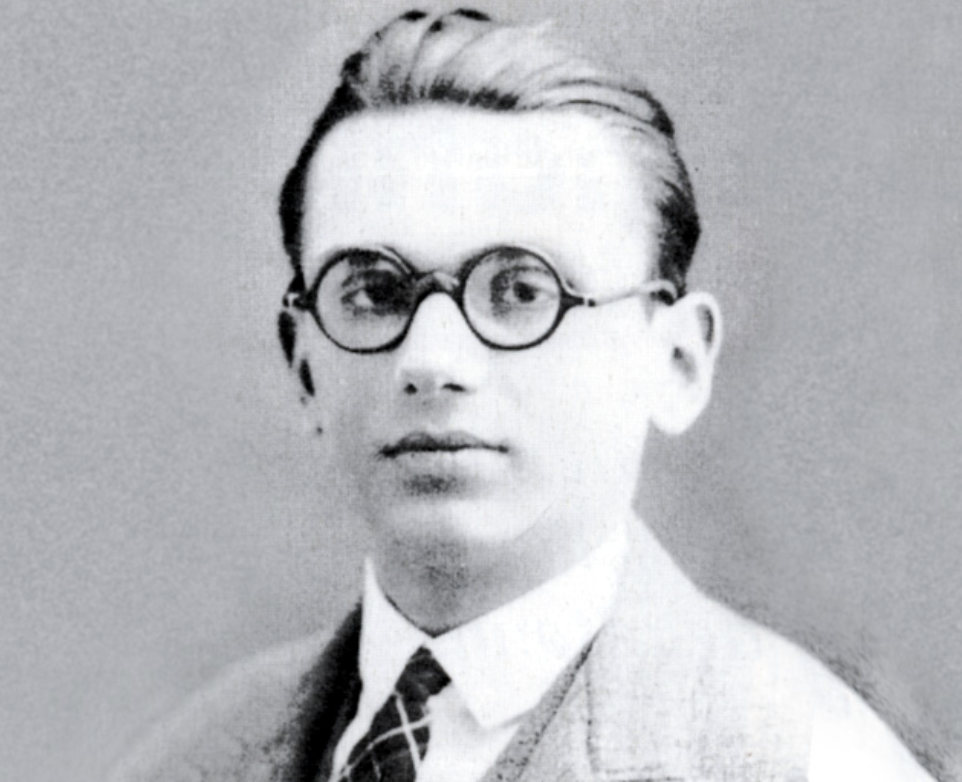
\includegraphics[scale=0.3]{Figures/godel.png}
     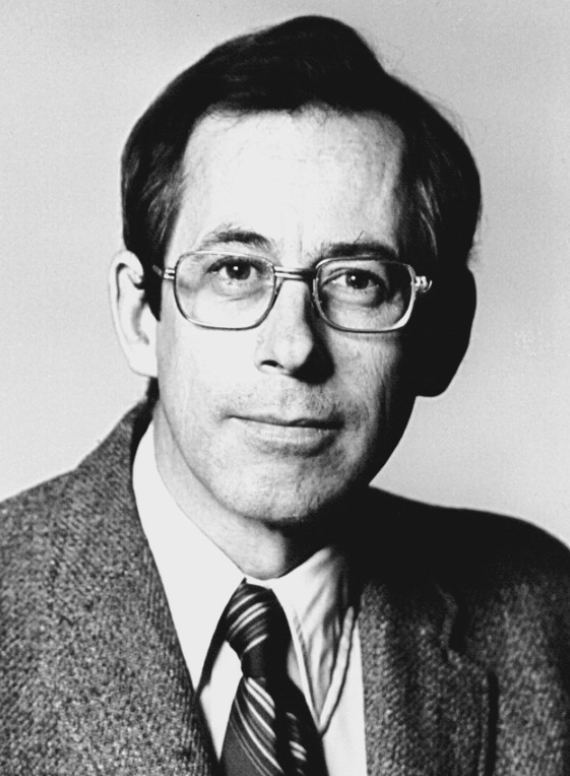
\includegraphics[scale=0.3]{Figures/peebles.png}
     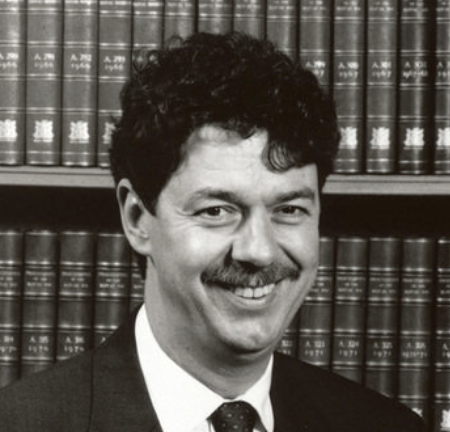
\includegraphics[scale=0.52]{Figures/sdmwhite.png}
  }
  \frame{
    \frametitle{Framework}
    \begin{itemize}
      \item Three angular momentum $J$ properties: 
      \item magnitude $|J|$: dominant discussion, ``angular momentum problem''
      \item headless direction ${\bf J J}$: aligned with tidal shear field
      \item sign of $J$: observable, thought to be in practice unpredictable
      \item Tidal Torque Theory (TTT) 
    \end{itemize}
  }
  \section{TTT}
  \frame{
    \frametitle{TTT}
    \begin{itemize}
      \item Neyrinck (2013), Yu et al (2017): Lagrangian Origami shapes of halos
      \item Lagrangian halos are not round, and will be torqued in
        linear theory
    \end{itemize}
      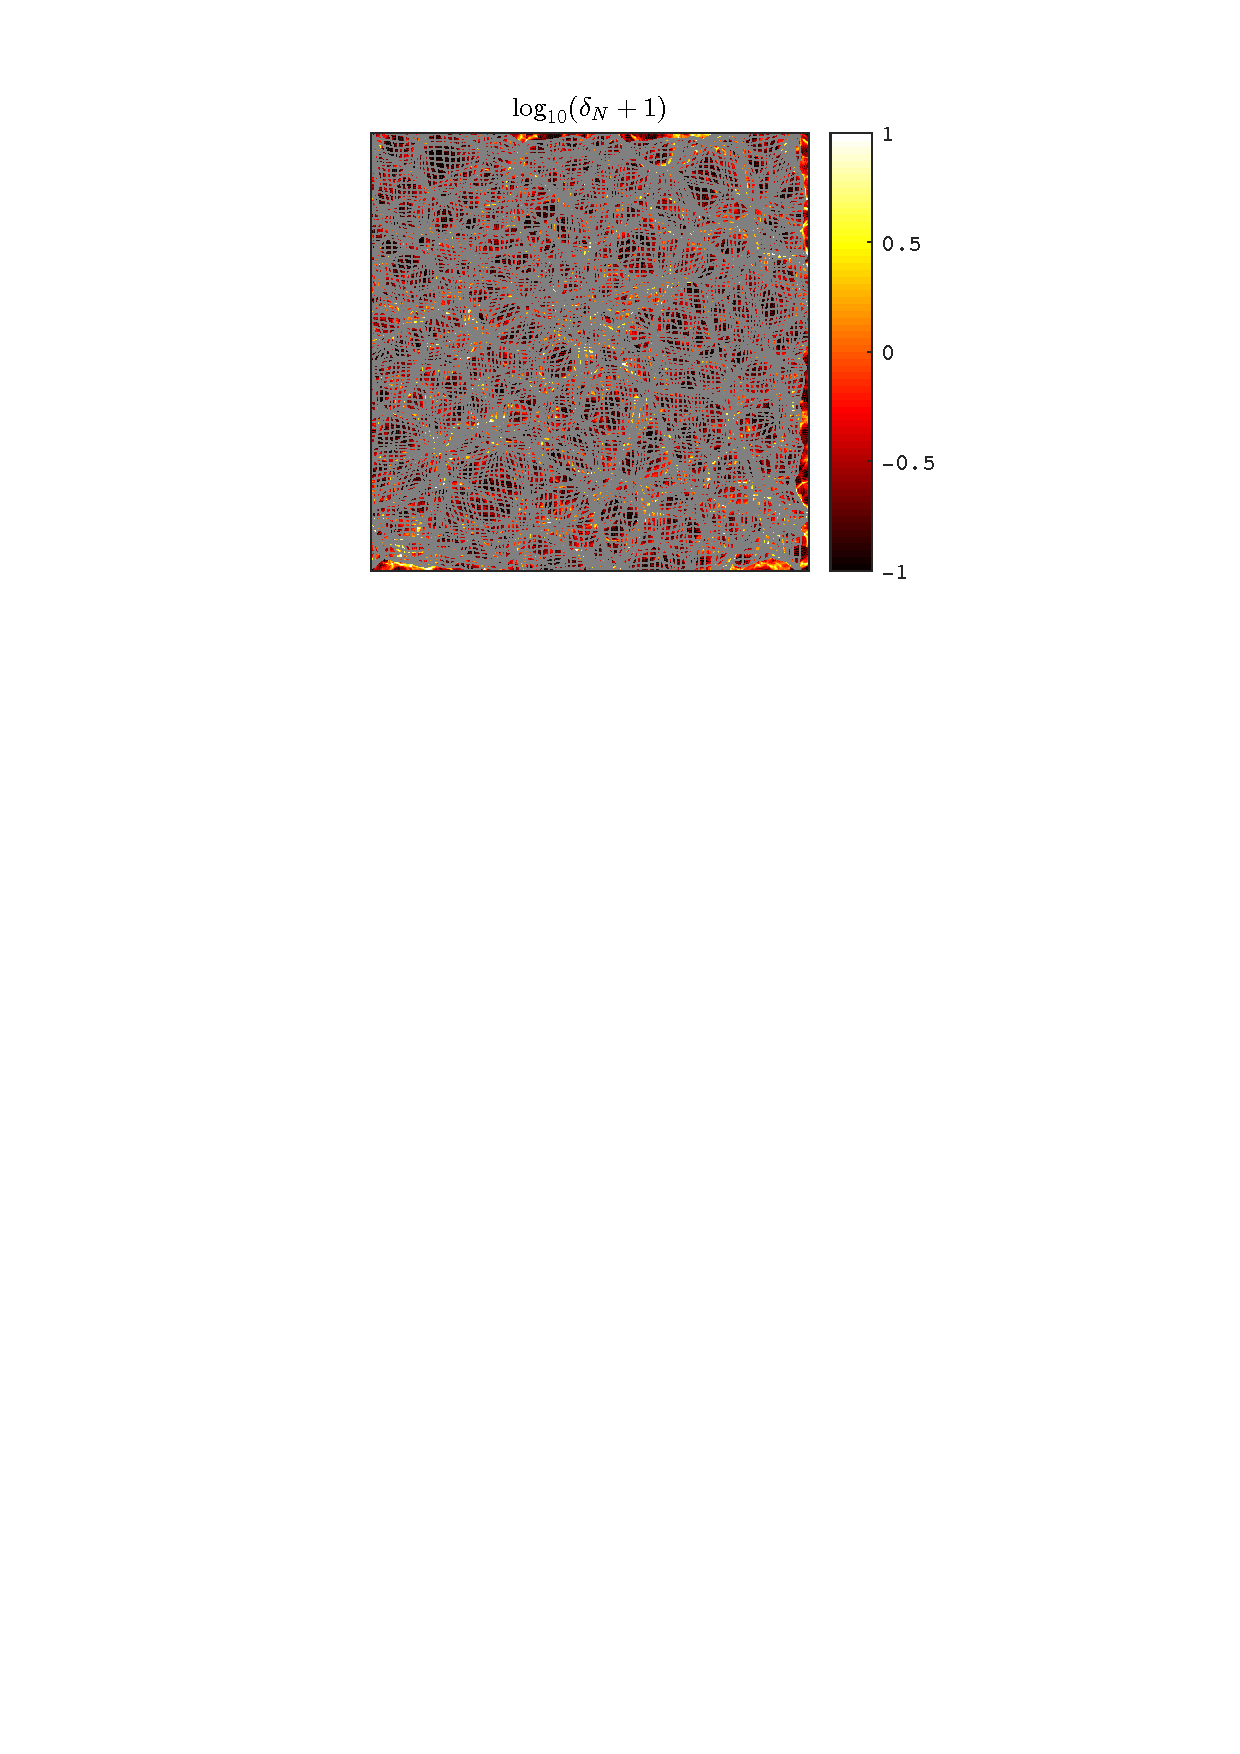
\includegraphics[scale=0.6]{Figures/rhoE.pdf}
      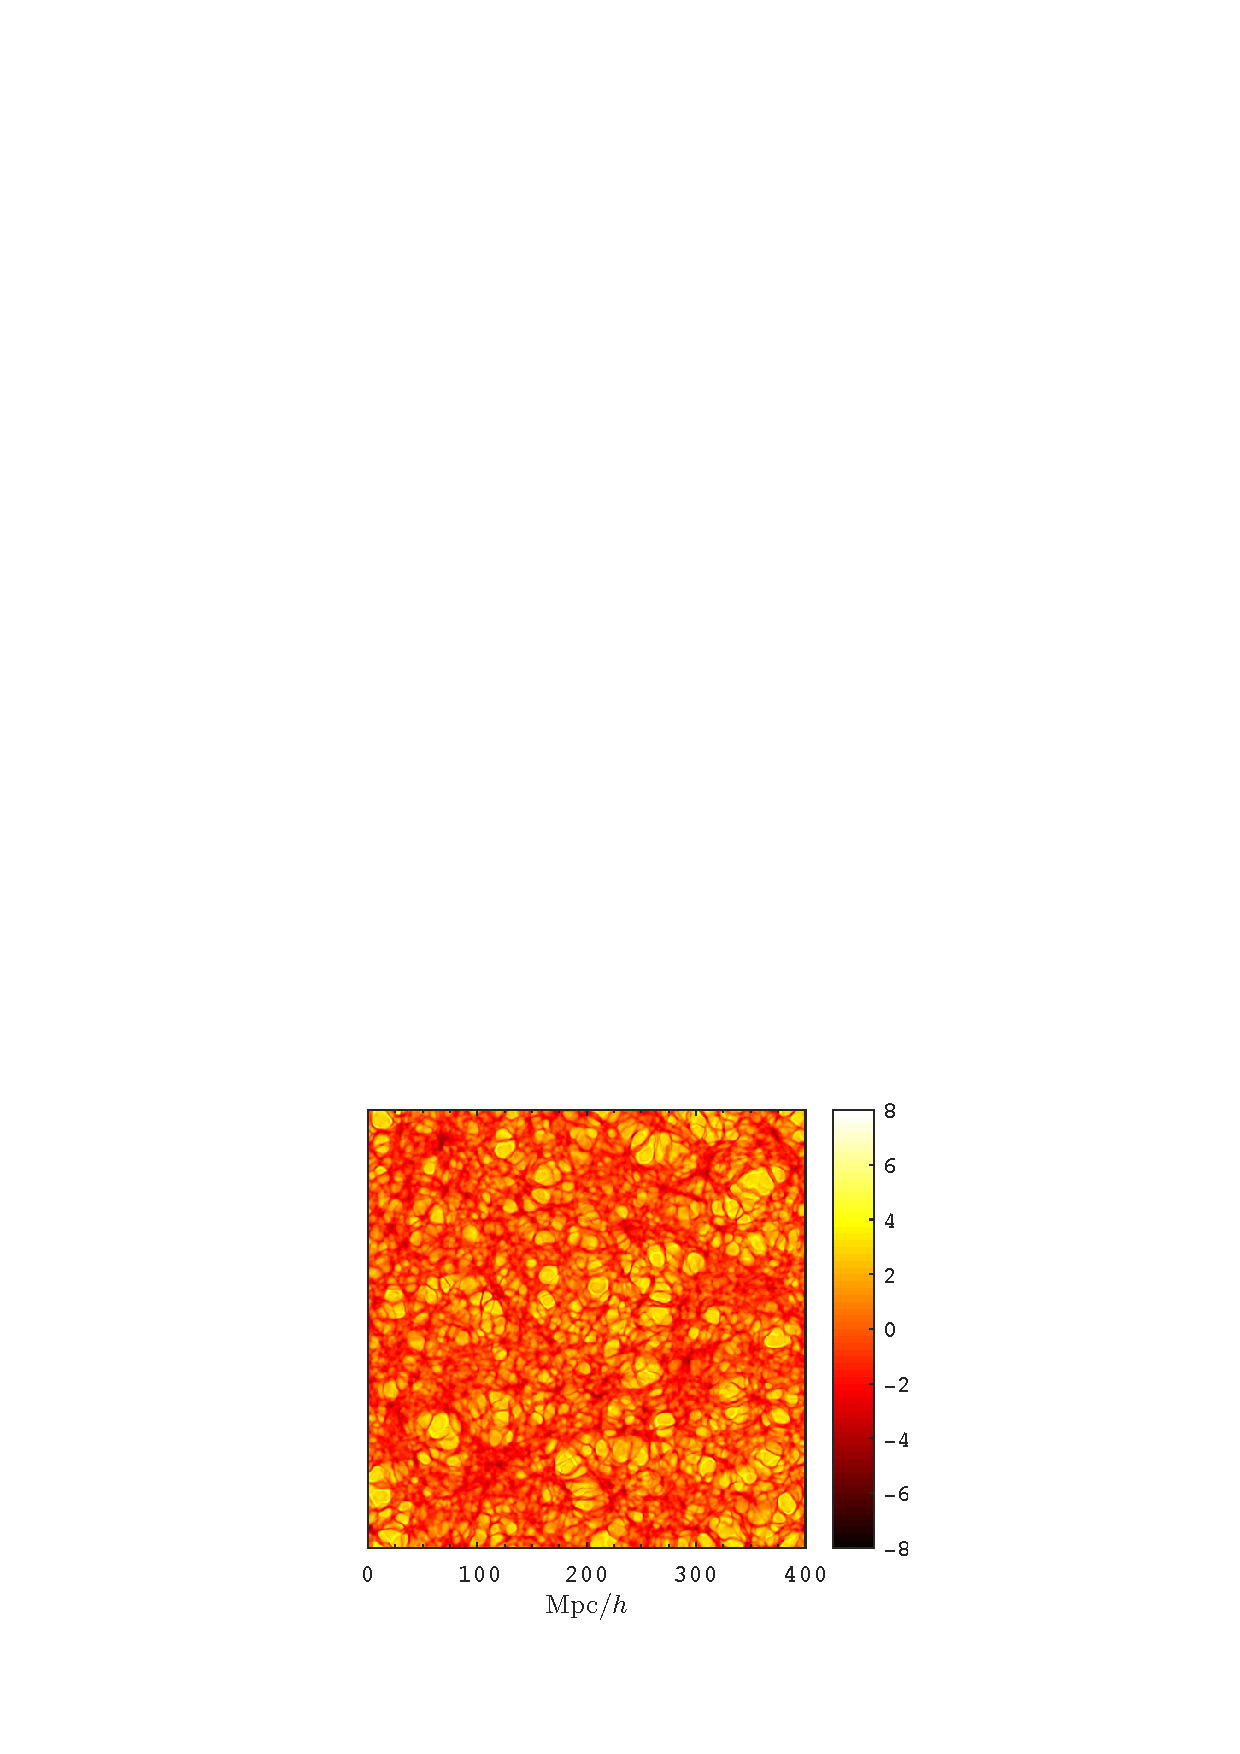
\includegraphics[scale=0.6]{Figures/rhoL.pdf}
  }

  \frame{
    \frametitle{In the beginning}
    \begin{itemize}
      \item torque $\tau = \int_\Omega {\bf F} \times {\bf r} \mathrm{d}^3x $
      \item moment of inertia tensor ${\bf I}_{ij}\equiv\int_\Omega x_i x_j\mathrm{d}^3x$
      \item external gravitational field $F_i=\partial_i
        \psi\sim x_j\partial_j\partial_i\psi\equiv x_j {\bf T}_{ij}$
      \item thus, $\tau_k = \epsilon_{ijk} {\bf T}_{lk}\int x_lx_i
        =\epsilon_{ijk} {\bf I}_{jl}{\bf T}_{lk}$
      \item linear TTT: inertia ${\bf I}$ constant, tide ${\bf
          T}\propto D \propto a$ grows as growth factor
    \end{itemize}
  }

 \frame{
    \frametitle{Knowns}
    \begin{itemize}
    \item Tidal field ${\bf T}$ well understood, studied, predicted
      and reconstructable from data (ELUCID, etc)
    \item inertia tensor ${\bf I}$: trivial to measure in simulations
      (lagrangian shape of halo), unclear how to reconstruct from data
    \item Zeldovich theory: $x=q+\nabla \phi$
      \item deformation tensor is tidal tensor with three eigenvalues $\lambda_i$
    \item halos are set of shell crossed particles $\lambda_i<-1$
    \item aligned with principal axis of small scale tidal tensor!
    \item two tidal effects: small scale determines ${\bf I}$, all
      larger scales ${\bf T}$
    \item halo particle self-gravity cannot self-torque
    \end{itemize}
  }


  \subsection{Conclusions}
  \frame{
    \frametitle{Conclusions}
    \begin{itemize}
    \item steady growth of understanding of TTT over half century
    \item new insights through simulations (Origami, Lagrangian)
    \item vast increase in observable data sets (SDSS++, zoo, ML, MANGA+)
    \item spins are quantitative fossils of smallest scale coherent
      observable structure 
    \item perhaps beginning of new era?
    \end{itemize}
  }
\end{document}
